%% =====================================================================
%%  Capítulo de L. Forzani, actualizado por la autora (2026-10) e integrado
%%  al apunte: preámbulo, macros y bibliografía viven en main.tex.
%% =====================================================================
\chapter{PCA y clasificación}\label{clas-cap}

% =====================================================================
\section{Introducción}\label{clas-sec:intro}

\textbf{Clasificar} es decidir a qué grupo pertenece una observación nueva, a
partir de un conjunto de observaciones de las que ya sabemos a qué grupo
pertenecen. Los grupos se llaman \textbf{clases} (en estadística se habla
también de \emph{poblaciones}). Por ejemplo: reconocer qué número es la imagen
de un dígito escrito a mano (diez clases: $0,1,\dots,9$), decidir si un tumor
es benigno o maligno a partir de mediciones de sus células, o distinguir un
colectivo de una camioneta por la forma de su silueta.

Los datos son, como en PCA, una matriz $X\in\R^{n\times p}$ con una
observación por fila ($\bi{x}_1\transp,\dots,\bi{x}_n\transp$, con $\bi{x}_i\in\R^p$) y una
variable por columna. La novedad es que ahora cada observación viene con una
\textbf{etiqueta}: un vector $y$ con $y_i\in\{1,\dots,C\}$, la clase de la
observación $i$. PCA no usaba las etiquetas; para clasificar, las vamos a usar.

En la práctica de este capítulo y del siguiente trabajamos con cuatro
conjuntos de datos:
\begin{center}
\small\renewcommand{\arraystretch}{1.15}
\begin{tabular}{lrrrp{6.2cm}}
datos & $n$ & $p$ & $C$ & qué se mide\\\hline
tumores de mama & $569$ & $30$ & $2$ & núcleos celulares en imágenes de punciones (maligno/benigno)\\
dígitos & $1797$ & $64$ & $10$ & intensidades de imágenes de $8\times8$ de dígitos escritos a mano\\
cáncer de pulmón & $32$ & $56$ & $3$ & atributos sin descripción, con valores enteros de $0$ a $3$ (tres tipos de cáncer)\\
siluetas de vehículos & $845$ & $18$ & $4$ & medidas de forma de la silueta (colectivo, camioneta, dos autos)
\end{tabular}
\end{center}
($n$ observaciones, $p$ variables, $C$ clases). Los dos primeros vienen con
\texttt{scikit-learn} y los dos últimos se bajan del repositorio UCI
\cite{UCI} (el de vehículos tiene $846$ filas, una de ellas incompleta, que
descartamos).

Este capítulo \textbf{no usa teoría estadística}: todo es geometría de
vectores y matrices. La idea central es muy simple: \emph{resumimos cada clase
con su media, y una observación nueva se asigna a la clase cuya media está más
cerca}. El plan:
\begin{enumerate}[leftmargin=*,itemsep=1pt]
\item la media de cada clase (Sección~\ref{clas-sec:medias});
\item la regla de la media más cercana, y cómo parte el espacio
(Sección~\ref{clas-sec:regla});
\item cómo se mide si un clasificador anda bien: entrenamiento y prueba
(Sección~\ref{clas-sec:evaluar}), y por qué importan las unidades
(Sección~\ref{clas-sec:escalas});
\item PCA antes de clasificar (Sección~\ref{clas-sec:pca}) y lo que PCA no ve
(Sección~\ref{clas-sec:nove}), que nos lleva al próximo capítulo.
\end{enumerate}
Hay clasificadores mucho más elaborados (ver, por ejemplo, \cite{HTF2009});
acá nos quedamos con el más simple.

% =====================================================================
\section{La media de cada clase}\label{clas-sec:medias}

Llamamos $n_k$ a la cantidad de observaciones de la clase $k$ (así que
$n_1+\dots+n_C=n$) y
\[
\bar{\bi{x}}_k=\frac1{n_k}\sum_{i:\ y_i=k}\bi{x}_i\ \in\R^p
\]
a la \textbf{media de la clase $k$}: el promedio, variable por variable, de las
filas de $X$ que son de la clase $k$. Es un punto de $\R^p$ que resume a toda
la clase. Como en el Capítulo~\ref{cap:pca}, $\bar{\bi{x}}=\frac1n\sum_{i=1}^n\bi{x}_i$ es la
media de todos los datos.

En los dígitos, cada observación es una imagen de $8\times8$ píxeles guardada
como un vector de $\R^{64}$, con una entrada por píxel (su intensidad de gris).
La media de la clase~3 es otro vector de $\R^{64}$ que, dibujado como imagen, es
un ``tres promedio'': borroso, pero se reconoce
(Figura~\ref{clas-fig:digitos-medias}).

\begin{figure}[htbp]
\centering
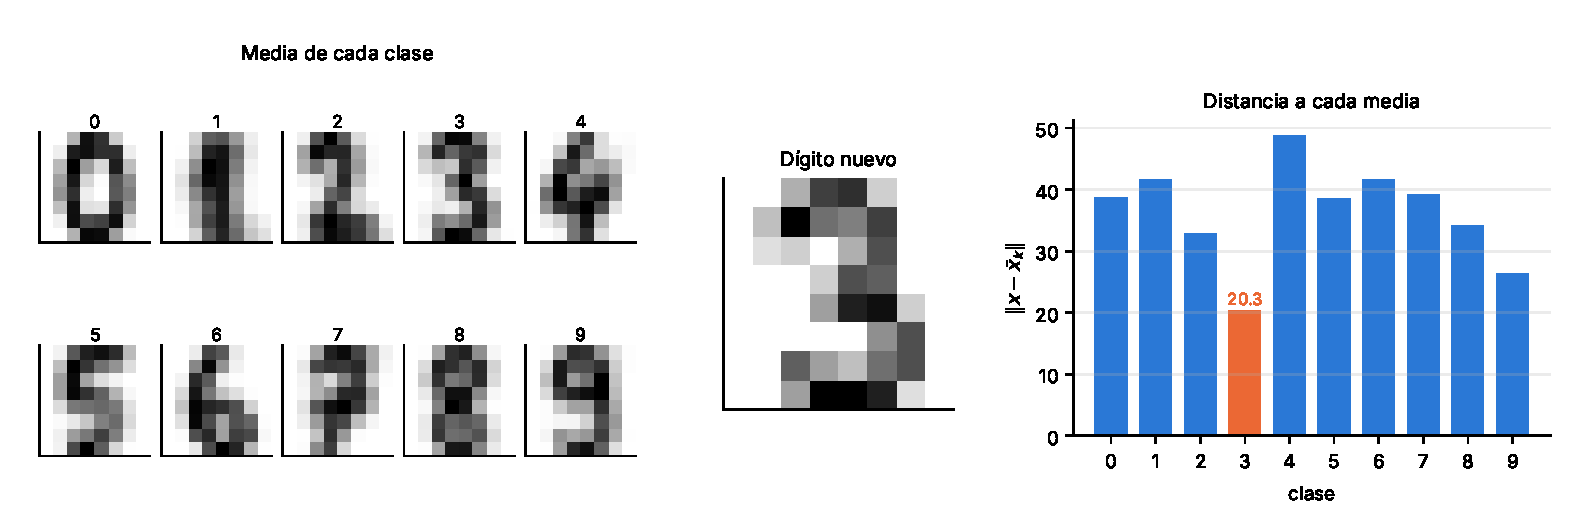
\includegraphics[width=\textwidth]{figuras/clasif_digitos_medias.pdf}
\caption{Dígitos escritos a mano (imágenes de $8\times8$ píxeles, así que
$p=64$). Izquierda: la media de cada una de las diez clases, calculada con
$1257$ imágenes de entrenamiento y dibujada como imagen. Centro: un dígito que
no se usó para calcular las medias. Derecha: su distancia a cada una de las
medias; la más chica es la distancia a la media de los treses.}
\label{clas-fig:digitos-medias}
\end{figure}

\begin{example}[Ocho puntos en el plano]\label{clas-ej:ocho}
Usamos este ejemplo en todo el capítulo y en el siguiente. La clase~1 son los
puntos $(2,3)$, $(1,3)$, $(-1,-3)$, $(-2,-3)$ y la clase~2 son $(5,3)$,
$(4,3)$, $(2,-3)$, $(1,-3)$: la segunda es la primera trasladada en $(3,0)$
(Figura~\ref{clas-fig:ocho}). Las medias de las clases son
\[
\bar{\bi{x}}_1=\tfrac14\bigl((2,3)+(1,3)+(-1,-3)+(-2,-3)\bigr)=(0,0),\qquad
\bar{\bi{x}}_2=(3,0),
\]
y la media de los ocho puntos es $\bar{\bi{x}}=(3/2,0)$.
\end{example}

\begin{remark}[Todas las medias con una multiplicación]\label{clas-rem:G}
Sea $G\in\R^{n\times C}$ la \textbf{matriz indicadora} de las clases:
$g_{ik}=1$ si la observación $i$ es de la clase $k$, y $g_{ik}=0$ si no. La
fila $k$ de $G\transp X$ es la suma de las filas de $X$ que son de la clase
$k$, y $G\transp G=\diag(n_1,\dots,n_C)$ (cada fila de $G$ tiene un solo uno,
así que sus columnas son ortogonales, y la columna $k$ tiene $n_k$ unos).
Entonces
\[
M=(G\transp G)^{-1}G\transp X\in\R^{C\times p}
\qquad\text{tiene en la fila $k$ a }\bar{\bi{x}}_k\transp .
\]
En los ocho puntos, ordenados como en el Ejemplo~\ref{clas-ej:ocho},
\begin{gather*}
G\transp=\begin{pmatrix}1&1&1&1&0&0&0&0\\0&0&0&0&1&1&1&1\end{pmatrix},\\[2pt]
G\transp G=\begin{pmatrix}4&0\\0&4\end{pmatrix},\qquad
G\transp X=\begin{pmatrix}0&0\\12&0\end{pmatrix},\qquad
M=\begin{pmatrix}0&0\\3&0\end{pmatrix}.
\end{gather*}
Así se calculan todas las medias a la vez en la computadora.
\end{remark}

% =====================================================================
\section{La regla de la media más cercana}\label{clas-sec:regla}

\begin{definition}[Clasificador de la media más cercana]\label{clas-def:regla}
Dadas las medias $\bar{\bi{x}}_1,\dots,\bar{\bi{x}}_C$ de las clases, una observación
nueva $\bi{x}\in\R^p$ se asigna a la clase cuya media está más cerca:
\[
f(\bi{x})=\argmin_{k=1,\dots,C}\ \|\bi{x}-\bar{\bi{x}}_k\| ,
\]
es decir, $f(\bi{x})$ es el $k$ para el que la distancia $\|\bi{x}-\bar{\bi{x}}_k\|$ es mínima.
(Si hay empate, se elige cualquiera de las clases empatadas; en la
computadora, la primera.)
\end{definition}

En la Figura~\ref{clas-fig:digitos-medias}, el dígito nuevo está a distancia
$20{,}3$ de la media de los treses y a más de $26$ de todas las demás: se lo
asigna a la clase~3, y efectivamente es un tres. ¿Cómo queda partido el
espacio entre las clases? Con dos clases la respuesta es sencilla.

\begin{proposition}[Con dos clases, la frontera es la mediatriz]\label{clas-prop:mediatriz}
Sean $\bi{a}\ne \bi{b}$ dos puntos de $\R^p$ (las medias de dos clases) y sea
$m=\frac12(\bi{a}+\bi{b})$ el punto medio entre ellos. Para todo $\bi{x}\in\R^p$,
\[
\|\bi{x}-\bi{a}\|^2-\|\bi{x}-\bi{b}\|^2=-2\,(\bi{a}-\bi{b})\transp(\bi{x}-m).
\]
En consecuencia, $\bi{x}$ está más cerca de $\bi{a}$ que de $\bi{b}$ si y solo si
$(\bi{a}-\bi{b})\transp(\bi{x}-m)>0$, y los puntos que están a la misma distancia de $\bi{a}$ y de
$\bi{b}$ forman el hiperplano
\[
\bigl\{\bi{x}\in\R^p:\ (\bi{a}-\bi{b})\transp(\bi{x}-m)=0\bigr\},
\]
que pasa por el punto medio $m$ y es perpendicular al segmento que une $\bi{a}$ con
$\bi{b}$. En el plano es la mediatriz del segmento, y en $\R^p$ también lo llamamos
así.
\end{proposition}

\begin{proof}
Desarrollando, $\|\bi{x}-\bi{a}\|^2=\|\bi{x}\|^2-2\bi{a}\transp \bi{x}+\|\bi{a}\|^2$, y lo mismo con $\bi{b}$. Al
restar se cancela $\|\bi{x}\|^2$:
\[
\|\bi{x}-\bi{a}\|^2-\|\bi{x}-\bi{b}\|^2=-2(\bi{a}-\bi{b})\transp \bi{x}+\|\bi{a}\|^2-\|\bi{b}\|^2 .
\]
Como $\bi{a}\transp \bi{b}=\bi{b}\transp \bi{a}$, se tiene $\|\bi{a}\|^2-\|\bi{b}\|^2=(\bi{a}-\bi{b})\transp(\bi{a}+\bi{b})=2(\bi{a}-\bi{b})\transp m$,
y queda $-2(\bi{a}-\bi{b})\transp \bi{x}+2(\bi{a}-\bi{b})\transp m=-2(\bi{a}-\bi{b})\transp(\bi{x}-m)$.
\end{proof}

Con dos clases, entonces, la regla de la media más cercana corta $\R^p$ en dos
semiespacios con un hiperplano: es un \emph{clasificador lineal}. Con más
clases, la clase $k$ gana en los puntos que están más cerca de $\bar{\bi{x}}_k$ que
de cada una de las otras medias; comparando de a dos con la
Proposición~\ref{clas-prop:mediatriz}, la región de la clase $k$ es la
intersección de $C-1$ semiespacios, y las fronteras son pedazos de mediatrices
(Ejercicios~\ref{clas-ej:tres} y~\ref{clas-ej:convexas}).

\begin{figure}[htbp]
\centering
\begin{tikzpicture}[scale=0.62]
  \fill[claseuno!7] (-3,-4) rectangle (1.5,4.2);
  \fill[clasedos!9] (1.5,-4) rectangle (6.2,4.2);
  \draw[->,gray!60] (-3,0)--(6.4,0) node[right]{\scriptsize $x_1$};
  \draw[->,gray!60] (0,-4)--(0,4.4) node[above]{\scriptsize $x_2$};
  \draw[thick,gray!80!black] (1.5,4.2)--(1.5,-4) node[below]{\scriptsize frontera: $x_1=3/2$};
  \foreach \x/\y in {2/3,1/3,-1/-3,-2/-3} {\fill[claseuno] (\x,\y) circle (4pt);}
  \foreach \x/\y in {5/3,4/3,2/-3,1/-3} {\fill[clasedos] ($(\x,\y)+(-4pt,-4pt)$) rectangle ++(8pt,8pt);}
  \draw[black,thick] (2,3) circle (8pt);
  \draw[black,thick] (1,-3) circle (8pt);
  \foreach \c/\x/\y in {claseuno/0/0,clasedos/3/0} {%
    \draw[black,line width=3.2pt] (\x-0.22,\y-0.22)--(\x+0.22,\y+0.22) (\x-0.22,\y+0.22)--(\x+0.22,\y-0.22);
    \draw[\c,line width=1.8pt] (\x-0.2,\y-0.2)--(\x+0.2,\y+0.2) (\x-0.2,\y+0.2)--(\x+0.2,\y-0.2);}
  \node[below left] at (0,0) {\scriptsize $\bar{\bi{x}}_1$};
  \node[below right] at (3,0) {\scriptsize $\bar{\bi{x}}_2$};
  \node[anchor=west] at (6.6,2.6) {\scriptsize \textcolor{claseuno}{$\bullet$} clase 1};
  \node[anchor=west] at (6.6,1.9) {\scriptsize \textcolor{clasedos}{$\blacksquare$} clase 2};
  \node[anchor=west] at (6.6,1.2) {\scriptsize $\times$ media de la clase};
  \node[anchor=west] at (6.6,0.5) {\scriptsize $\bigcirc$ mal clasificado};
\end{tikzpicture}
\caption{Los ocho puntos del Ejemplo~\ref{clas-ej:ocho} y las medias de las
dos clases. La regla de la media más cercana corta el plano por la mediatriz
de las medias (la recta $\bi{x}_1=3/2$) y se equivoca en los dos puntos marcados.}
\label{clas-fig:ocho}
\end{figure}

\begin{example}[La media más cercana en los ocho puntos]\label{clas-ej:ocho-regla}
En el Ejemplo~\ref{clas-ej:ocho}, la mediatriz de $\bar{\bi{x}}_1=(0,0)$ y
$\bar{\bi{x}}_2=(3,0)$ es la recta $\bi{x}_1=3/2$: todo punto con $\bi{x}_1<3/2$ va a la
clase~1, y todo punto con $\bi{x}_1>3/2$, a la clase~2. El punto $(2,3)$ de la
clase~1 y el punto $(1,-3)$ de la clase~2 quedan del lado equivocado, así que
la regla acierta $6$ de los $8$ puntos (Figura~\ref{clas-fig:ocho}). Mirando el
dibujo, las clases se pueden separar perfectamente con una recta inclinada. La
regla no la encuentra porque solo mira las medias y no la forma de las clases,
que son alargadas. En el próximo capítulo (LDA, análisis discriminante lineal)
vamos a encontrar esa recta.
\end{example}

% =====================================================================
\section{Entrenar y probar}\label{clas-sec:evaluar}

¿Cómo sabemos si un clasificador anda bien? Contar los aciertos sobre los
mismos datos con los que calculamos las medias es hacer trampa: el
clasificador ya ``vio'' esos datos, y el resultado suele ser demasiado
optimista. Lo que interesa es cómo le va con datos \emph{nuevos}. Por eso,
antes de empezar, los datos se separan al azar en dos partes:
\begin{itemize}[leftmargin=*,itemsep=1pt]
\item los de \textbf{entrenamiento}, $(X_{\text{ent}},y_{\text{ent}})$, con los
que se calcula \emph{todo} lo que el clasificador necesita: las medias de las
clases y, más adelante, los desvíos para estandarizar y las direcciones de
PCA;
\item los de \textbf{prueba}, $(X_{\text{pru}},y_{\text{pru}})$, que se guardan
y se usan una sola vez, al final, para contar los aciertos.
\end{itemize}
Lo habitual es separar un $70\%$ para entrenar y un $30\%$ para probar,
manteniendo en las dos partes la proporción de cada clase (separación
\emph{estratificada}) y con una \emph{semilla} fija (el número con el que
arranca el generador de números al azar), para que el resultado se pueda
repetir.

\begin{definition}[Aciertos y matriz de confusión]\label{clas-def:confusion}
Supongamos que el clasificador les asigna las clases $\hat y_1,\dots,\hat y_m$
a las $m$ observaciones de prueba, cuyas clases verdaderas son
$y_1,\dots,y_m$. La proporción de \textbf{aciertos} es la proporción de las
observaciones con $\hat y_i=y_i$, y el \textbf{error} es uno menos la
proporción de aciertos. La \textbf{matriz de confusión} es $K\in\R^{C\times C}$ con
\[
K_{jk}=\text{cantidad de observaciones de la clase $j$ asignadas a la clase $k$}.
\]
En la diagonal están los aciertos, así que la proporción de aciertos es
$\tr(K)/m$.
\end{definition}

\begin{example}[Tumores de mama]\label{clas-ej:mama-confusion}
Con las variables estandarizadas (Sección~\ref{clas-sec:escalas}), la regla de
la media más cercana clasifica así a los $171$ tumores de prueba (filas: clase
verdadera; columnas: clase asignada; primero maligno y después benigno):
\[
K=\begin{pmatrix}56&8\\7&100\end{pmatrix}.
\]
Acierta $56+100=156$ de $171$, el $91{,}2\%$. Pero la matriz muestra más: de
los $64$ tumores malignos, $8$ fueron clasificados como benignos, que en
medicina es el error más grave. La matriz de confusión dice \emph{qué} se confunde con
qué, y no solo cuánto.
\end{example}

\begin{mdframed}[linewidth=0.8pt,linecolor=gray]
\noindent\textbf{Receta: cómo se clasifica} (vale para cualquier clasificador)
\begin{enumerate}[leftmargin=*,itemsep=1pt]
\item \textbf{Separar} los datos en entrenamiento y prueba.
\item \textbf{Entrenar}: con los datos de entrenamiento, calcular todo lo que
haga falta (medias y desvíos para estandarizar, las direcciones de PCA, las
medias de las clases).
\item \textbf{Probar}: a $X_{\text{pru}}$ aplicarle \emph{las mismas}
transformaciones, con los números del paso~2 (sin recalcularlos), clasificar y
comparar con $y_{\text{pru}}$: aciertos y matriz de confusión.
\item \textbf{Usar}: una observación nueva se trata igual que una de prueba.
\end{enumerate}
\end{mdframed}

\begin{remark}[Con pocos datos]\label{clas-rem:pocos}
Con los $32$ pacientes de cáncer de pulmón, la prueba tiene solo $10$, y el
porcentaje de aciertos puede cambiar mucho según cómo haya caído la separación
al azar. En ese caso conviene repetir la separación con varias semillas y
mirar todos los resultados (Ejercicio~\ref{clas-ej:semillas}).
\end{remark}

% =====================================================================
\section{Las unidades importan}\label{clas-sec:escalas}

El cuadrado de la distancia euclídea suma las diferencias al cuadrado de todas
las variables por igual. Si una variable varía mucho más que las otras (si
tiene un desvío mucho mayor), domina la distancia.

En los datos de vinos (otro conjunto clásico, que también viene con
\texttt{scikit-learn}: $178$ vinos, $13$ variables químicas y $3$ variedades
de uva), la variable \emph{prolina} tiene, en el entrenamiento, un desvío de
$327$, y todas las demás tienen desvíos menores que $15$: la varianza de la
prolina es el $99{,}8\%$ de la suma de las varianzas de las $13$ variables. La
regla de la media más cercana usa entonces prácticamente solo la prolina: en
los $54$ vinos de prueba asigna exactamente las mismas clases que si
miráramos únicamente esa variable, y acierta el $68{,}5\%$.
\textbf{Estandarizando}, es decir, restando la media y dividiendo por el
desvío de cada variable (los dos calculados con el entrenamiento), acierta el
$98{,}1\%$. En los tumores de mama pasa lo mismo en menor escala: $87{,}7\%$
sin estandarizar y $91{,}2\%$ estandarizando (las dos áreas de los núcleos,
con desvíos de $578$ y $364$, dominan a todas las demás variables).

En forma matricial, estandarizar es reemplazar cada $\bi{x}$ por
\[
D^{-1}(\bi{x}-\bar{\bi{x}}),\qquad D=\diag(s_1,\dots,s_p),
\]
con la media $\bar{\bi{x}}$ y los desvíos $s_j$ de las variables calculados con el
entrenamiento: es cambiar las unidades de cada variable. Las distancias
cambian, y con ellas pueden cambiar las clases asignadas
(Ejercicio~\ref{clas-ej:invariancias}). Estandarizar no siempre es mejor: si
todas las variables ya están en la misma escala, como los píxeles de una
imagen, puede empeorar las cosas (Ejercicio~\ref{clas-ej:pixeles}). En el
próximo capítulo, LDA va a elegir la manera de medir distancias teniendo en
cuenta la forma de las clases.

% =====================================================================
\section{PCA antes de clasificar}\label{clas-sec:pca}

Con muchas variables ($64$ píxeles, $30$ mediciones) es natural reducir
primero la dimensión con PCA y clasificar en $\R^d$, con $d$ chico:
\begin{enumerate}[leftmargin=*,itemsep=1pt]
\item con los datos de entrenamiento, calcular la media $\bar{\bi{x}}$ (y, si hace
falta, estandarizar) y la SVD de la matriz centrada, $X_c=U\Sigma V\transp$;
quedarse con $V_d$, las primeras $d$ columnas de $V$;
\item reemplazar cada observación $\bi{x}$ (de entrenamiento o de prueba) por sus
$d$ scores $z=V_d\transp(\bi{x}-\bar{\bi{x}})\in\R^d$;
\item clasificar $z$ con la regla de la media más cercana en $\R^d$.
\end{enumerate}
Para el paso~3 hacen falta las medias de las clases en las coordenadas
nuevas, y no hay que calcular nada más: como los scores se obtienen restando
$\bar{\bi{x}}$ y multiplicando por $V_d\transp$, la media de los scores de la clase
$k$ es el score de la media,
\[
\frac1{n_k}\sum_{i:\ y_i=k}V_d\transp(\bi{x}_i-\bar{\bi{x}})
=V_d\transp\Bigl(\frac1{n_k}\sum_{i:\ y_i=k}\bi{x}_i-\bar{\bi{x}}\Bigr)
=V_d\transp(\bar{\bi{x}}_k-\bar{\bi{x}}).
\]
Lo primero que conviene saber es que, si no truncamos, no perdemos nada.

\begin{proposition}[Con todas las componentes no cambia nada]\label{clas-prop:todas}
Si $d=p$, es decir, si usamos la matriz ortogonal $V\in\R^{p\times p}$ con
todos los vectores singulares derechos, entonces para todo $\bi{x}\in\R^p$ y toda
clase $k$,
\[
\bigl\|V\transp(\bi{x}-\bar{\bi{x}})-V\transp(\bar{\bi{x}}_k-\bar{\bi{x}})\bigr\|=\|\bi{x}-\bar{\bi{x}}_k\| .
\]
Por lo tanto, la regla de la media más cercana con los $p$ scores asigna las
mismas clases que con las variables originales.
\end{proposition}

\begin{proof}
$V\transp(\bi{x}-\bar{\bi{x}})-V\transp(\bar{\bi{x}}_k-\bar{\bi{x}})=V\transp(\bi{x}-\bar{\bi{x}}_k)$, y una
matriz ortogonal conserva las longitudes:
$\|V\transp \bi{u}\|^2=\bi{u}\transp VV\transp \bi{u}=\bi{u}\transp \bi{u}=\|\bi{u}\|^2$.
\end{proof}

Pasar a las coordenadas de PCA es solo llevar el origen a $\bar{\bi{x}}$ y girar los
ejes (y tal vez reflejar alguno), y eso no cambia las distancias. Si la matriz
centrada tiene rango $r<p$, alcanza con sus $r$ primeras componentes: tampoco
cambia nada (Ejercicio~\ref{clas-ej:rango}). Eso pasa si hay más variables que
datos, o si hay variables constantes: en los dígitos de entrenamiento hay
cuatro píxeles que valen siempre $0$, y $r=60$. Lo
que sí cambia las cosas es \emph{truncar}, quedarse con $d$ componentes cuando
hay más: se pierden las coordenadas en las direcciones $\bi{v}_{d+1},\bi{v}_{d+2},\dots$,
las distancias a las medias se achican, cada una de manera distinta, y la
clase asignada puede cambiar. A veces es para bien (se descarta ``ruido'') y
muchas veces para mal.

\begin{figure}[htbp]
\centering
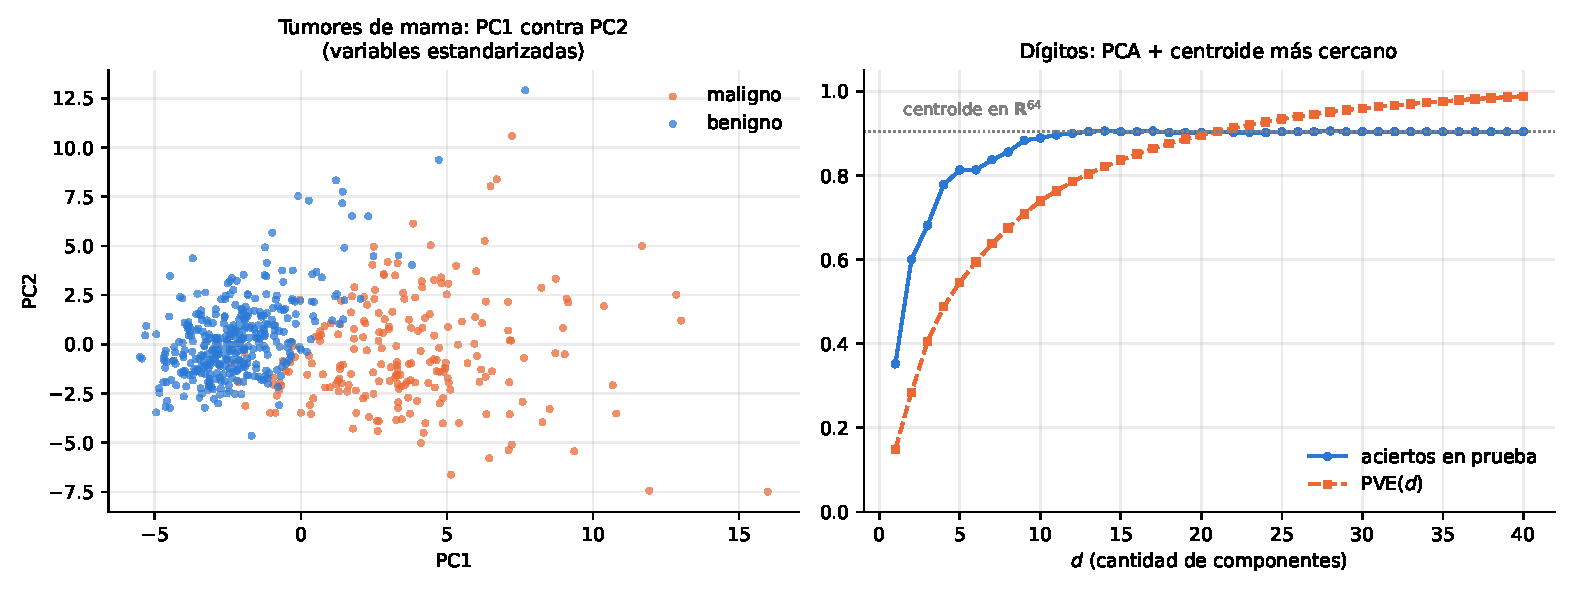
\includegraphics[width=\textwidth]{figuras/clasif_pca_mama_digitos.pdf}
\caption{Izquierda: las dos primeras componentes principales de los $569$
tumores de mama (todos los datos, con las variables estandarizadas; entre
paréntesis, la proporción de la varianza que explica cada una); las clases ya
se distinguen bastante en PC1. Derecha: dígitos (sin estandarizar); proporción
de aciertos en prueba de la media más cercana calculada en $\R^d$ con los
scores de PCA, junto con la proporción de varianza explicada $\PVE(d)$ por las
primeras $d$ componentes (definida en el Capítulo~\ref{cap:pca}).}
\label{clas-fig:pca-mama-digitos}
\end{figure}

La Figura~\ref{clas-fig:pca-mama-digitos} muestra dos situaciones típicas. En
los tumores de mama (estandarizados), la primera componente principal ya
separa bastante bien las clases: con $d=1$, la regla de la media más cercana
acierta el $90{,}1\%$ de los tumores de prueba, y con $d\ge4$ se llega al
$91{,}2\%$ que se obtiene con las $30$ variables. En los dígitos, con $d=2$ se
acierta apenas el $60\%$ (los dos primeros scores sirven para dibujar, pero no
alcanzan para clasificar), con $d=10$ el $88{,}9\%$ y con $d=20$ el $90{,}2\%$,
casi lo mismo que en $\R^{64}$ ($90{,}4\%$). Observemos que la curva de
aciertos se estabiliza mucho antes que la de varianza explicada (a partir de
$d=10$ mejora muy poco, y $\PVE(10)$ es apenas del $74\%$): \emph{explicar
varianza y clasificar bien no son lo mismo}.

\paragraph{Mirar antes de clasificar.} El gráfico de PC1 contra PC2 con los
puntos coloreados por clase es una muy buena primera mirada a un conjunto de
datos con muchas variables, y muchas veces muestra más que cualquier par de
variables originales (aunque, como vamos a ver enseguida, puede esconder
justo la dirección que separa las clases). Es el punto~\ref{clas-p:pca} de la
práctica.

% =====================================================================
\section{Lo que PCA no ve}\label{clas-sec:nove}

PCA elige sus direcciones \emph{sin mirar las etiquetas}: busca las
direcciones en las que los datos, todos juntos, varían más. Para clasificar,
en cambio, queremos direcciones en las que las clases proyectadas queden
\emph{separadas}, y nada garantiza que sean las de máxima varianza.

\begin{example}[PCA en los ocho puntos]\label{clas-ej:ocho-pca}
Centrando los ocho puntos del Ejemplo~\ref{clas-ej:ocho} (recordemos que
$\bar{\bi{x}}=(3/2,0)$), la matriz de covarianza es
\[
S=\frac17\begin{pmatrix}38&36\\36&72\end{pmatrix},
\]
con autovalores $\lambda_1\approx13{,}54$ y $\lambda_2\approx2{,}17$ y
direcciones principales $\bi{v}_1\approx(0{,}535;\,0{,}845)$ y
$\bi{v}_2\approx(0{,}845;\,-0{,}535)$. La primera explica el $86\%$ de la
varianza ($\PVE(1)\approx0{,}86$): la nube de los ocho puntos es alargada en
la dirección de $\bi{v}_1$, igual que cada clase (Figura~\ref{clas-fig:ocho-pca}).

Si reducimos a $d=1$ con PCA, los scores $\bi{v}_1\transp(\bi{x}_i-\bar{\bi{x}})$ de la clase~1
son $2{,}80$; $2{,}27$; $-3{,}87$; $-4{,}41$, y los de la clase~2 son
$4{,}41$; $3{,}87$; $-2{,}27$; $-2{,}80$: las clases quedan completamente
mezcladas. Las medias de los scores son $-0{,}80$ y $0{,}80$, y la regla de la
media más cercana en la recta acierta $4$ de los $8$ puntos, como si
tiráramos una moneda.

En cambio, los scores sobre la segunda dirección, $\bi{v}_2\transp(\bi{x}_i-\bar{\bi{x}})$,
son $-1{,}18$; $-2{,}03$; $-0{,}51$; $-1{,}35$ en la clase~1 y $1{,}35$;
$0{,}51$; $2{,}03$; $1{,}18$ en la clase~2: todos negativos en una clase y
todos positivos en la otra. Las clases quedan perfectamente separadas, y la
regla de la media más cercana sobre $\bi{v}_2$ acierta los $8$ puntos (¡mejor que
en todo el plano, donde acertaba $6$!). La dirección que separa las clases es
justamente la de varianza \emph{chica}, la que PCA descarta. Mirando el plano
se entiende por qué: la recta que pasa por $\bar{\bi{x}}$ en la dirección de $\bi{v}_1$
deja a cada clase de un lado, y lo que distingue a las clases es de qué lado de
esa recta están, es decir, el signo de su coordenada sobre $\bi{v}_2$.
\end{example}

\begin{figure}[!htb]
\centering
\begin{tikzpicture}[scale=0.47]
  % ---- el plano, con las direcciones principales dibujadas desde la media
  \draw[->,gray!60] (-3,0)--(6.2,0) node[right]{\scriptsize $x_1$};
  \draw[->,gray!60] (0,-4)--(0,4.3) node[above]{\scriptsize $x_2$};
  \draw[dashed,gray] ($(1.5,0)-4.4*(0.535,0.845)$)--($(1.5,0)+4.4*(0.535,0.845)$);
  \foreach \x/\y in {2/3,1/3,-1/-3,-2/-3} {\fill[claseuno] (\x,\y) circle (4pt);}
  \foreach \x/\y in {5/3,4/3,2/-3,1/-3} {\fill[clasedos] ($(\x,\y)+(-4pt,-4pt)$) rectangle ++(8pt,8pt);}
  \draw[-{Stealth},very thick,black] (1.5,0)--($(1.5,0)+2.3*(0.535,0.845)$) node[left]{\scriptsize $v_1$};
  \draw[-{Stealth},very thick,black] (1.5,0)--($(1.5,0)+2.3*(0.845,-0.535)$) node[right]{\scriptsize $v_2$};
  \fill[black] (1.5,0) circle (3pt);
  \node[anchor=east,font=\scriptsize] at (1.35,0.35) {$\bar{\bi{x}}$};
  \node[anchor=west] at (7,2.2) {\scriptsize \textcolor{claseuno}{$\bullet$} clase 1};
  \node[anchor=west] at (7,1.5) {\scriptsize \textcolor{clasedos}{$\blacksquare$} clase 2};
\end{tikzpicture}

\smallskip
\begin{tikzpicture}[x=1.25cm,y=1cm]
  % ---- los scores sobre v1 y sobre v2 (la raya punteada es el punto medio entre las medias)
  \foreach \yy/\tit/\uno/\dos/\mu in {%
      0/{scores sobre $v_1$, la dirección de máxima varianza: se mezclan ($4$ de $8$)}/{2.80,2.27,-3.87,-4.41}/{4.41,3.87,-2.27,-2.80}/0.80,%
      -1.95/{scores sobre $v_2$, la dirección de varianza chica: se separan ($8$ de $8$)}/{-1.18,-2.03,-0.51,-1.35}/{1.35,0.51,2.03,1.18}/1.27} {%
    \begin{scope}[yshift=\yy cm]
      \draw[gray!60] (-4.8,0)--(4.8,0);
      \foreach \t in {-4,-2,0,2,4} {\draw[gray!60] (\t,-0.1)--(\t,0.1);
        \node[below,gray,font=\tiny] at (\t,-0.12) {$\t$};}
      \draw[gray,densely dashed] (0,-0.3)--(0,0.95);
      \foreach \t in \uno {\fill[claseuno] (\t,0) circle (2.6pt);}
      \foreach \t in \dos {\fill[clasedos] ($(\t,0)+(-2.6pt,-2.6pt)$) rectangle ++(5.2pt,5.2pt);}
      \foreach \c/\t in {claseuno/-\mu,clasedos/\mu} {%
        \draw[black,line width=2.6pt] (\t-0.13,0.42)--(\t+0.13,0.74) (\t-0.13,0.74)--(\t+0.13,0.42);
        \draw[\c,line width=1.4pt] (\t-0.115,0.44)--(\t+0.115,0.72) (\t-0.115,0.72)--(\t+0.115,0.44);}
      \node[anchor=south,font=\scriptsize] at (0,0.95) {\tit};
    \end{scope}}
\end{tikzpicture}
\caption{Arriba: los ocho puntos y sus direcciones principales, dibujadas
desde la media $\bar{\bi{x}}$; la recta punteada pasa por $\bar{\bi{x}}$ en la dirección de
$\bi{v}_1$. Abajo: los scores de cada punto sobre $\bi{v}_1$ y sobre $\bi{v}_2$, con la media
de los scores de cada clase ($\times$); la raya punteada es el punto medio
entre las dos medias, la frontera de la regla de la media más cercana en la
recta.}
\label{clas-fig:ocho-pca}
\end{figure}

La explicación es que la varianza en una dirección mezcla dos cosas: cuánto se
desparrama cada clase alrededor de su media, y cuánto se separan entre sí las
medias de las clases. Para clasificar solo sirve lo segundo; lo primero
estorba. PCA no puede distinguirlas porque no mira las etiquetas, y en los
ocho puntos casi toda la varianza en la dirección de $\bi{v}_1$ es dispersión de
cada clase alrededor de su media. En el próximo capítulo, \textbf{LDA} va a
buscar directamente, usando las etiquetas, la dirección en la que las medias de las clases quedan lo más
separadas posible en relación con lo que se desparrama cada clase.

% =====================================================================
% \section*{Videos}   % COMPLETAR si hay videos de este capítulo

% =====================================================================
\begin{ideas}[frametitle={Ideas clave},frametitlefont=\bfseries\large,frametitlebelowskip=4pt]
\begin{itemize}[leftmargin=*,itemsep=2pt]
\item \textbf{Clasificar}: asignar una clase a una observación nueva, usando
datos cuyas clases conocemos (la matriz $X$ y el vector de etiquetas $y$).
\item \textbf{La media de cada clase}, $\bar{\bi{x}}_k$, resume a la clase con un
punto. Todas a la vez: $M=(G\transp G)^{-1}G\transp X$.
\item \textbf{La media más cercana}: se asigna la clase cuya media está más
cerca. Con dos clases, la frontera es el hiperplano que pasa por el punto
medio entre las medias y es perpendicular al segmento que las une (la
mediatriz).
\item \textbf{Entrenar y probar}: todo se calcula con el entrenamiento y se
mide con la prueba; la matriz de confusión dice qué clases se confunden.
\item \textbf{Las unidades importan}: una variable con un desvío mucho mayor
que las otras domina la distancia; estandarizar (con los desvíos del
entrenamiento) lo corrige.
\item \textbf{PCA antes de clasificar}: con todas las componentes no cambia
nada ($V$ es ortogonal); truncar sí cambia. Explicar varianza no es lo mismo
que clasificar bien.
\item \textbf{PCA no mira las etiquetas}: la dirección de máxima varianza
puede mezclar las clases, y la que las separa puede ser de varianza chica. LDA
busca esa dirección.
\end{itemize}
\end{ideas}

% =====================================================================
\section*{Ejercicios}
\addcontentsline{toc}{section}{Ejercicios}

\noindent\footnotesize \textsc{[Cálculo]} para fijar la mecánica,
\textsc{[Concepto]} para justificar y demostrar, \textsc{[Datos]} para la
computadora.\normalsize

\begin{enumerate}[leftmargin=*,label=\textbf{\thechapter.\arabic*},ref=\thechapter.\arabic*,itemsep=4pt]

\item \tipo{Cálculo} \textbf{Tres clases a mano.}\label{clas-ej:tres} La clase
A son los puntos $(0,0),(2,0),(0,2),(2,2)$; la clase B, $(5,0),(7,0),(5,2),(7,2)$;
y la clase C, $(2,5),(4,5),(2,7),(4,7)$.
\begin{enumerate}[label=(\alph*)]
\item Calcular las medias de las tres clases y la media de los doce puntos.
Escribir la matriz indicadora $G$ y verificar que $(G\transp G)^{-1}G\transp X$
tiene a las medias en las filas.
\item Escribir las ecuaciones de las tres mediatrices y dibujar las regiones
de la media más cercana. ¿Por qué las tres mediatrices se cortan en un mismo
punto?
\item Clasificar los puntos $(3,3)$, $(4,3)$ y $(4,4)$.
\end{enumerate}

\item \tipo{Concepto} \textbf{Las regiones son convexas.}\label{clas-ej:convexas}
Sea $R_k$ el conjunto de los $\bi{x}\in\R^p$ que están más cerca de $\bar{\bi{x}}_k$ que
de todas las otras medias.
\begin{enumerate}[label=(\alph*)]
\item Usando la Proposición~\ref{clas-prop:mediatriz}, escribir $R_k$ como
intersección de $C-1$ semiespacios.
\item Deducir que si $\bi{x}$ y $\bi{x}'$ están en $R_k$, todo el segmento que los une
está en $R_k$.
\end{enumerate}

\item \tipo{Concepto} \textbf{Todas las distancias de una vez.}\label{clas-ej:distancias}
Sean $X_{\text{nueva}}\in\R^{m\times p}$, con filas $\bi{u}_1\transp,\dots,\bi{u}_m\transp$
(las observaciones que queremos clasificar), y $M\in\R^{C\times p}$, con las
medias de las clases en las filas. Sea $\Delta\in\R^{m\times C}$ la matriz con
$\Delta_{ik}=\|\bi{u}_i-\bar{\bi{x}}_k\|^2$.
\begin{enumerate}[label=(\alph*)]
\item Probar que $\Delta=\bi{a}\,\mathbf 1_C\transp-2X_{\text{nueva}}M\transp+\mathbf 1_m\,c\transp$,
donde $a_i=\|\bi{u}_i\|^2$, $c_k=\|\bar{\bi{x}}_k\|^2$, y $\mathbf 1_C$, $\mathbf 1_m$ son
vectores de unos.
\item Deducir que la clase asignada a $\bi{u}_i$ es el $k$ que hace máximo
$\bar{\bi{x}}_k\transp \bi{u}_i-\frac12\|\bar{\bi{x}}_k\|^2$, que es una función lineal de $\bi{u}_i$
más una constante.
\end{enumerate}

\item \tipo{Cálculo} \textbf{La matriz de confusión.}\label{clas-ej:confusion}
\begin{enumerate}[label=(\alph*)]
\item Diez observaciones de prueba tienen las clases verdaderas $y$, y el
clasificador les asigna las clases $\hat y$:
\[
y=(1,1,1,2,2,2,3,3,3,3),\qquad \hat y=(1,1,2,2,2,3,3,3,1,3).
\]
Calcular la matriz de confusión, la proporción de aciertos y la proporción de
aciertos dentro de cada clase.
\item Si $G$ y $\widehat G$ son las matrices indicadoras de las clases
verdaderas y de las asignadas, probar que $K=G\transp\widehat G$, que la suma
de la fila $j$ de $K$ es la cantidad de observaciones de la clase $j$, y que
el clasificador acierta todo si y solo si $K$ es diagonal.
\end{enumerate}

\item \tipo{Concepto} \textbf{¿Qué cosas no cambian la clase asignada?}\label{clas-ej:invariancias}
A todos los datos, los de entrenamiento y los nuevos, se les aplica la misma
transformación. ¿Cambia la clase que asigna la regla de la media más cercana
si la transformación es una traslación $\bi{x}\mapsto \bi{x}+c$? ¿Y si es $\bi{x}\mapsto Q\bi{x}$,
con $Q$ ortogonal? ¿Y si se multiplica una sola de las variables por $10$? Dar
un ejemplo en $\R^2$, con dos clases de dos puntos cada una, en el que
estandarizar cambie la clase asignada a un punto nuevo.

\item \tipo{Concepto} \textbf{Cuando la matriz centrada no tiene rango
completo.}\label{clas-ej:rango} Sea $X_c$ la matriz de entrenamiento centrada,
de rango $r<p$ (por ejemplo, porque hay más variables que datos); sean
$\bi{v}_1,\dots,\bi{v}_r$ sus primeros $r$ vectores singulares derechos,
$V_r=[\bi{v}_1\cdots \bi{v}_r]$ y $P=V_rV_r\transp$.
\begin{enumerate}[label=(\alph*)]
\item Probar que cada $\bar{\bi{x}}_k-\bar{\bi{x}}$ es combinación lineal de las filas de
$X_c$, y que por lo tanto está en $\gen(\bi{v}_1,\dots,\bi{v}_r)$.
\item Probar que $(I-P)(\bi{x}-\bar{\bi{x}}_k)=(I-P)(\bi{x}-\bar{\bi{x}})$, que no depende de $k$,
y deducir que
$\|\bi{x}-\bar{\bi{x}}_k\|^2=\|V_r\transp(\bi{x}-\bar{\bi{x}}_k)\|^2+\|(I-P)(\bi{x}-\bar{\bi{x}})\|^2$.
\item Concluir que la regla de la media más cercana con los $r$ scores asigna
las mismas clases que en $\R^p$.
\item Truncar sí puede cambiar las cosas: mostrar con los ocho puntos del
Ejemplo~\ref{clas-ej:ocho} (donde $r=p=2$) que con $d=1$ cambian algunas de
las clases asignadas (comparar con el Ejemplo~\ref{clas-ej:ocho-pca}).
\end{enumerate}

\item \tipo{Cálculo} \textbf{Máxima varianza no es máxima separación.}\label{clas-ej:dos-rectas}
La clase~1 son los puntos $(-3,0)$, $(-1,0)$, $(1,0)$, $(3,0)$ y la clase~2 son
$(-3,1)$, $(-1,1)$, $(1,1)$, $(3,1)$.
\begin{enumerate}[label=(\alph*)]
\item Centrar los ocho puntos, calcular la matriz de covarianza, $\bi{v}_1$ y
$\PVE(1)$, y proyectar las dos clases sobre $\bi{v}_1$. ¿Se distinguen? ¿Sobre qué
dirección sí se distinguen, y cuánto vale la varianza de los datos en esa
dirección?
\item Clasificar los ocho puntos con la media más cercana en $\R^2$. Después
reducir a $d=1$ con PCA: ¿qué les pasa a las medias de las dos clases en la
recta? ¿Se pueden clasificar los puntos?
\item Explicar por qué maximizar la varianza no garantiza separar las clases:
¿qué información no usa PCA?
\end{enumerate}

\item \tipo{Datos} \textbf{¿Conviene estandarizar los píxeles?}\label{clas-ej:pixeles}
En los dígitos, comparar los aciertos de la media más cercana y de PCA $+$
media más cercana, con y sin estandarizar. ¿Qué pasa con los píxeles que
valen siempre $0$ en el entrenamiento? ¿Por qué estandarizar puede empeorar
las cosas en imágenes?

\item \tipo{Datos} \textbf{¿Cuánto depende de la separación?}\label{clas-ej:semillas}
Repetir $20$ veces la separación $70/30$, con las semillas $0,1,\dots,19$, y
calcular cada vez los aciertos en prueba de la media más cercana. Hacerlo con
los tumores de mama (estandarizados) y con el cáncer de pulmón (cuyas
variables ya están todas en la misma escala), y comparar los veinte resultados de cada uno (mínimo, máximo,
histograma). ¿Por qué varían tanto más con el cáncer de pulmón?

\item \tipo{Datos} \textbf{Los dígitos promedio.} Con los dígitos de
entrenamiento, calcular las diez medias y dibujarlas como imágenes de
$8\times8$ (Figura~\ref{clas-fig:digitos-medias}). Clasificar los dígitos de
prueba con la media más cercana, mirar la matriz de confusión y dibujar
algunos dígitos mal clasificados al lado de la media de su clase y de la media
de la clase que se les asignó. ¿Qué dígitos se confunden más? ¿Se entiende
por qué?

\end{enumerate}

% =====================================================================
\section*{Práctica: clasificar con PCA}
\addcontentsline{toc}{section}{Práctica: clasificar con PCA}
% =====================================================================

Los datos de la práctica son los cuatro conjuntos de la
Sección~\ref{clas-sec:intro}: tumores de mama, dígitos, cáncer de pulmón y
siluetas de vehículos (son los de la notebook \texttt{Datos\_PCA.ipynb} de la
cátedra, pero acá se cargan con un archivo de Python). Cada grupo trabaja con
el conjunto que se le asigne. El objetivo es investigar si es posible predecir
la clase a partir de las variables, y qué se gana y qué se pierde al reducir la
dimensión con PCA. El informe se entrega en una notebook de Colab con el
código, los gráficos (con ejes y títulos) y las respuestas a cada punto,
escritas en celdas de texto. Junto con la notebook se distribuyen dos archivos
de Python: \texttt{datos\_clasificacion.py}, que carga los cuatro conjuntos ya
limpios, y \texttt{herramientas\_clasificacion.py}, con funciones auxiliares;
para usarlos en Colab basta subirlos y hacer \texttt{import}.

\begin{enumerate}[leftmargin=*,label=\textbf{P.\arabic*},ref=P.\arabic*,itemsep=6pt]

\item \textbf{Investigación preliminar.} Busque información sobre su conjunto
de datos y conteste: ¿en qué consisten los datos? ¿Cuál es el objetivo de la
clasificación? ¿Cuántos predictores hay? Describa las variables (si hay
información sobre ellas).
Notación: $X\in\R^{n\times p}$ es la matriz cuyas filas son los individuos y
cuyas columnas son las características medidas, e $y$ es el vector con la
clase de cada individuo.

\item \textbf{Cargar y describir.} Cargue los datos con
\begin{center}
\texttt{X, y, variables, clases = cargar("mama")}
\end{center}
(o \texttt{"digitos"}, \texttt{"pulmon"}, \texttt{"vehiculos"}). Informe $n$, $p$, $C$ y cuántos
individuos hay en cada clase. ¿Había datos faltantes en el archivo original?
(Lea la descripción de \texttt{cargar} en \texttt{datos\_clasificacion.py}.) ¿Las
variables están en escalas parecidas? (Mire los desvíos de las columnas.)

\item \textbf{Gráficos exploratorios.} Elija pares de variables (pares de
columnas de $X$) y haga gráficos de dispersión con los puntos coloreados según
la clase. Etiquete los ejes.

\item \textbf{PCA.}\label{clas-p:pca} Centre los datos (y estandarícelos si
las escalas son muy distintas; justifique) y calcule PCA con la SVD.
\begin{itemize}[itemsep=1pt]
\item Grafique los valores singulares y $\PVE(d)$.
\item Grafique PC1 contra PC2 con los puntos coloreados por clase y los ejes
etiquetados.
\item Mire las entradas de $\bi{v}_1$ y $\bi{v}_2$: ¿qué variables pesan más?
\item ¿Qué gráfico permite ver mejor las clases, los pares de variables o las
componentes principales? ¿Por qué?
\end{itemize}

\item \textbf{Entrenamiento y prueba.} Lea la receta de la
Sección~\ref{clas-sec:evaluar}. Separe los datos en entrenamiento ($70\%$) y
prueba ($30\%$), de manera estratificada y con una semilla fija
(\texttt{separar(X, y)}). De acá en adelante, todo lo que se calcule (medias,
desvíos, $V_d$, medias de las clases) se calcula con el entrenamiento. Con el
cáncer de pulmón, repita además todo con otras semillas
(Observación~\ref{clas-rem:pocos}).

\item \textbf{La media más cercana.} Calcule los aciertos en entrenamiento y
en prueba de la regla de la media más cercana en $\R^p$, con y sin
estandarizar, y la matriz de confusión en prueba. ¿Qué clases se confunden
más?

\item \textbf{PCA $+$ media más cercana.} Para $d=1,2,\dots$ (hasta el rango
de la matriz centrada de entrenamiento, o hasta $40$), reduzca a $d$
componentes y clasifique con la media más cercana en $\R^d$. Grafique los
aciertos en prueba junto con $\PVE(d)$. ¿Con cuántas componentes conviene
quedarse? (Elegir $d$ mirando los datos de prueba es hacer un poco de trampa,
porque la prueba debería usarse una sola vez; acá lo aceptamos por
simplicidad.) Verifique que con todas las componentes se obtiene lo mismo que
en $\R^p$ (Proposición~\ref{clas-prop:todas} y Ejercicio~\ref{clas-ej:rango}).

\item \textbf{Conclusiones.} ¿Qué usaría para clasificar sus datos, y con
cuántas componentes? ¿Es cierto que ``explicar más varianza'' significa
``clasificar mejor''? ¿Qué información no usa PCA?

\end{enumerate}

\subsection*{Los archivos de Python}

\begin{itemize}[leftmargin=*,itemsep=2pt]
\raggedright
\item \texttt{datos\_clasificacion.py}: \texttt{cargar(nombre)} devuelve
\texttt{X, y, variables, clases} para \texttt{"mama"}, \texttt{"digitos"},
\texttt{"pulmon"} y \texttt{"vehiculos"} (las etiquetas $y$ son enteros
$0,\dots,C-1$). Arregla la lectura del cáncer de pulmón (el archivo está
separado por comas, la clase es la \emph{primera} columna y hay cinco datos
faltantes, marcados con \texttt{?}, que se reemplazan por la mediana de su
columna). Incluye \texttt{separar(X, y, prop\_prueba=0.3, semilla=0)}, una
separación estratificada.
\item \texttt{herramientas\_clasificacion.py}: \texttt{estandarizar},
\texttt{columnas\_no\_constantes}, \texttt{pca\_svd}, \texttt{scores} (proyecta
datos nuevos con la media y la $V_d$ del entrenamiento), \texttt{medias} (las
medias de las clases, una por fila), \texttt{clasificar\_media} (la regla de la
media más cercana), \texttt{matriz\_confusion}, \texttt{aciertos} y dos
funciones de gráficos. (El archivo trae también las funciones que se usan en
el Capítulo~\ref{lda-cap}.)
\end{itemize}
% PARA EL DOCENTE (no se distribuye): practica10_pca_clasificacion.py es una
% resolución completa de la práctica; "python practica10_pca_clasificacion.py mama"
% guarda los gráficos en resultados_mama/ y escribe los resultados.

% =====================================================================
